\chapter{Performance Evaluation}
Now we’ll walk through a practical, systematic way to evaluate the performance of any systems — especially networking protocols — and we’ll explain the decision points you’ll meet: what to measure, how to measure it, what trade-offs you’re making, and how to present the results.

\section{Practical steps}
\begin{enumerate}
    \item Begin by writing down the question you want the evaluation to answer. For example, you might want to compare a brand new MAC protocol for sensor networks against the current standard. Saying that aloud helps avoid wasting time. Be specific about what “better” means in your context: is it lower energy consumption, higher packet delivery ratio, lower latency, or longer network lifetime? Often you want a mix of those.
    \item Next list the concrete services your system provides and the outcomes you’ll observe. For a MAC protocol the service is simple: nodes send packets to their neighbors. The outcomes you can directly observe are whether each packet was delivered successfully, how long it took, how much energy was spent to send or receive it, and whether the network is still alive after a long period.
\end{enumerate}
Your evaluation will rest on a handful of performance metrics. Common ones for sensor-network MAC protocols include latency, packet delivery ratio (PDR), energy consumption, and network lifetime.
\textit{Parameters} are things you have to set for the system: number of nodes, duty cycle, transmission power, and so on. \textit{Factors} are the subset of parameters you will vary deliberately in your experiments so you can see how the system behaves.
    
There are three broad ways to evaluate performance.
\begin{itemize}
    \item \textit{Analytical modeling} uses math to derive performance formulas or bounds. It’s fast and cheap but requires simplifying assumptions; if you want a quick insight or to explore parameter relationships, modeling is excellent.
    \item \textit{Simulation} builds a virtual version of the system in software and runs experiments with controllable randomness and repeatability. It captures more detail than analytic models and is relatively inexpensive, but results depend on the simulator’s fidelity.
    \item \textit{Measurement} (running on real hardware) gives results in the real world, but it’s costly in time, money, and logistics. Measurement can reveal issues simulations missed, but it’s vulnerable to uncontrolled environmental variation.
\end{itemize}
Which one to choose depends on where you are in the lifecycle, how much time and money you have, what tools you can access, and how accurate you need to be.
If your system is brand new and you don’t have hardware, modeling or simulation are essentially your only choices. If you already have a prototype, measurements become an option and often a necessity.
If you need results extremely quickly, analytical modeling tends to be fastest because it often requires only pencil, paper, and some math. If you can afford a bit more time, simulation provides richer, more realistic results.

Analytical models are cheap and quick but often less accurate because of simplifying assumptions. Simulations are more costly but can include more system details and therefore usually produce results closer to reality. Measurements cost the most in terms of equipment and time, but they’re easiest to convince stakeholders with.

Think through these aspects as you plan.
\begin{itemize}
    \item \textit{Stage:} Are you evaluating a conceptual design, a prototype, or a production-ready system? Early stage favors modeling or simulation.
    \item \textit{Time:} How quickly do you need answers? Tight deadlines push toward analytic modeling and careful approximations.
    \item \textit{Tools:} What existing modeling, simulation, or measurement tools do you or your lab have? Use what you know unless there’s a compelling reason to learn a new tool.
    \item \textit{Accuracy:} How precise must the results be to support your claim? If small differences matter, you’ll need simulations or measurements.
    \item \textit{Trade-}off evaluation: Do you need to compare many designs or parameter settings? Modeling can let you explore broad spaces cheaply.
    \item \textit{Cost:} What budget is available for hardware, testbeds, or researcher time? Balance ambition against resources.
    \item \textit{Sellability:} Who needs to be convinced? If your audience is skeptical, measurement results can be more convincing than equations or simulation traces.
\end{itemize}

Designing experiments means deciding which factors to vary and how, what workloads to run, and which combinations of settings give you the most information with minimal effort.
\begin{enumerate}
    \setcounter{enumi}{2}
    \item Start by choosing a baseline — a fixed set of parameter values that represent a realistic or commonly used configuration. Then create a small set of experiments that explore meaningful deviations from that baseline, focusing on the factors you think will matter most.

    \item Workload selection is often overlooked, but it can make or break your study. Workload describes the traffic patterns and events that occur during the experiment: how many flows, where they start and end, packet sizes, and inter-arrival times. Choose workloads that mimic real application scenarios your protocol is intended for.

    \item Once you have data, plotting is your friend. Don’t hide the variance: reporting means without variability is misleading. When comparing two protocols, determine whether observed differences are statistically significant and practically meaningful.

    \item When preparing plots and tables, make them answer the question you set out at the start. 
    Explain what the observed trade-offs mean for a system designer. For example, “Protocol A reduces average energy per packet by 20\% compared to Protocol B when inter-arrival times are long, but at high traffic loads Protocol A’s packet delivery drops sharply due to collisions.”

    Finally, be transparent about limitations. Discuss what you did not model, what assumptions you made, and how those might affect the conclusions.
\end{enumerate}

\section{Three rules of validation}
\begin{enumerate}
    \item \textit{Do not trust a simulation result until you validate it against either an analytical model or measurements.} Simulators can have bugs or unrealistic parameters.
    \item \textit{Do not trust an analytical model until you validate it with simulation or measurement.} Models make simplifying assumptions that can hide important behavior.
    \item \textit{Do not trust a measurement until you validate it with an analytical model or a simulation.} Real systems have noise and unique environmental factors; cross-checking helps you separate systemic behavior from artifacts.
\end{enumerate}

\section{Selecting performance metrics}
When you evaluate something you’re essentially asking: does it do the job I want, and how well? To answer that you need to observe outcomes and summarize them with metrics that people understand and trust. Good metrics make your results comparable, reproducible, and useful for decision making. Bad metrics hide important trade-offs and can mislead.

When a system is asked to perform a service, there are three high-level outcomes. It can succeed and do the service correctly, it can do it incorrectly (an error), or it can refuse/fail to perform the service at all (unavailable).

These three outcomes are important because they suggest three kinds of metrics you should track: metrics that describe \textit{speed} (how fast successful services complete), metrics that describe \textit{reliability} (how often incorrect behaviors occur, and what kinds of errors), and metrics that describe \textit{availability} (how often the system refuses or fails).

\begin{figure}[ht]
    \centering
    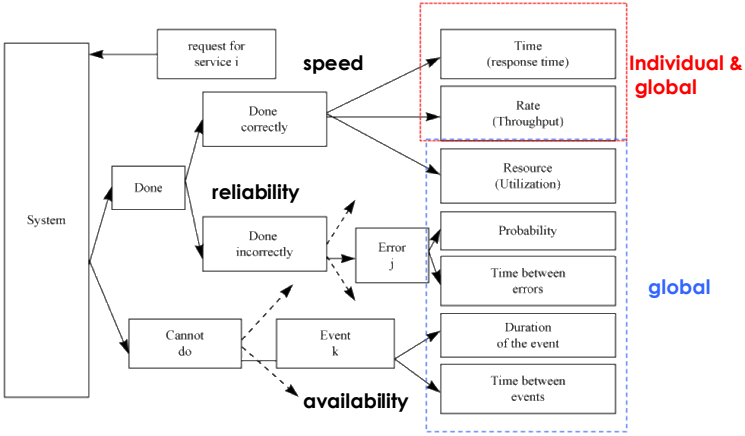
\includegraphics[width=0.8\linewidth]{images/performance-metrics.png}
    \caption{Selecting performance metrics.}
    \label{fig:performance-metrics}
\end{figure}

\subsection{Speed, reliability, availability}
If the service is performed correctly, we measure:
\begin{itemize}
    \item \textit{Speed:} how long the service takes. For a packet, this is latency: the time between packet arrival and its successful delivery (or acknowledgment).
    \item \textit{Productivity:} how many services are completed per unit time. For a gateway, throughput is the number of packets forwarded per second.
    \item \textit{Utilization:} what fraction of system resources are busy serving requests. For a gateway this could be CPU busy time, radio on time, or channel occupancy as a percentage of elapsed time.
\end{itemize}
If the system performs incorrectly, errors occur. It helps to classify different error types and measure their probabilities. For a gateway you might measure single-bit errors, whole packet corruption, misrouting, etc., and estimate the fraction of packets in each error class.

If the system fails or is unavailable, classify the failure modes (hardware failure, software crash, network partition) and estimate how often each mode happens. For example, the gateway may be unavailable 0.01\% of the time due to processor failure and 0.03\% due to software failure.

A network is shared by multiple users, which means there are two perspectives to measure performance.
\begin{itemize}
    \item An individual metric tells how well the system serves one user or one flow — user-centric utility. Examples are per-user throughput, per-flow latency, or per-node energy consumption.
    \item A global metric captures the system-wide utility — total throughput across all users, fairness indices, or aggregate energy consumed by the whole network.
\end{itemize}
Optimizing for an individual metric doesn’t always optimize the global metric. A classic example is throughput: a single user grabbing the channel aggressively may improve their own throughput but lower others’ throughput so much that total throughput or fairness gets worse.

Lots of metrics are possible, and many are correlated. Two useful principles when selecting which metrics to report are non-redundancy and completeness.
\begin{itemize}
    \item \textit{Non-redundancy} means don’t report metrics that say the same thing in slightly different words. If two measures convey essentially the same information, pick the clearer one.
    \item \textit{Completeness} means your metric set should collectively reflect all possible outcomes: success (speed/productivity/utilization), error (reliability), and unavailability (availability). If you ignore one of those outcomes you may miss important behavior.
\end{itemize}

\begin{Example}{Evaluating a new MAC protocol}{}
    You design a new MAC protocol for wireless sensor networks and want to show it’s better than existing protocols. You choose simulation as the evaluation technique (because you probably don’t have hardware yet), implement the protocol in the simulator, choose a scenario and workload (number of nodes, traffic pattern), pick metrics, run multiple repeated simulations varying some parameters, and get a pile of numbers.

    What now? You have to summarize and present the measured data in a way that speaks clearly to the question: “Is the new MAC better, and under what conditions?”
\end{Example}

\section{Summarizing measured data}
A measurement campaign can generate hundreds, thousands, or millions of observations for any variable (latency, energy per packet, throughput, etc.). You’ll rarely want to dump raw values into a paper or report. Instead you summarize central tendency and variability, and use figures that make comparisons obvious.

\subsection{Summarizing data by a single number}
Two questions are central: how to summarize a dataset by a single number that is meaningful, and how to summarize its variability so readers understand the confidence or spread.

\subsubsection{Empirical mean}
The most common single-number summary is the \textit{empirical mean}. Given observations $x_1,x_2,\ldots,x_n$, the sample mean is the sum of the observations divided by $n$:
\begin{equation*}
    \bar{x}=\frac{1}{n}\sum_{i=0}^nx_i.
\end{equation*}
For many variables and large enough samples with limited skew, the mean is informative. But remember: the mean is only a summary; it can be misleading when data are highly skewed or have extreme outliers.

Suppose you measured two packet latencies: one was $l_1=2$ ms and the other $l_2=5$ s. Be careful with units. The mean is 
\begin{equation*}
    \frac{(0.002+5)}{2}=\frac{5.002}{2}=2.501 s
\end{equation*}
Reporting “mean latency = 2.501 seconds” is correct arithmetically, but it’s useless as a description of the system because the two observations reflect two very different behaviors (one very short, one very long).

\subsubsection{Geometric mean}
If your performance numbers are multiplicative improvements (factors like “2$\times$ faster”, “0.5$\times$ energy”), the \textit{geometric mean} is a more appropriate average because it treats multiplicative changes symmetrically. For numbers $x_1,x_2\ldots,x_n$ the geometric mean is
\begin{equation*}
    \frac{\prod_{i=1}^nx_i}{n}.    
\end{equation*}

\subsection{Summarizing variability}
Knowing the mean without variability is dangerous. Two systems may have the same mean but very different consistency. Usually you prefer the system whose performance is predictable and low variance.

Common measures of dispersion are range, variance/standard deviation, coefficient of variation, and percentiles (quantiles). Each has pros and cons.

\subsubsection{Range}
Range is the difference between the maximum and minimum observed values. It’s simple to compute and sometimes useful when you know the variable is bounded. But range is highly sensitive to outliers and sample size: as you collect more samples, the maximum tends to get larger (if the tail is unbounded), making range unstable. Use range only when you have reason to believe the variable is bounded or when min/max themselves are meaningful.

\subsubsection{Variance and Standard deviation}
Variance measures the average squared deviation from the mean:
\begin{equation*}
        s^2 = \frac{1}{n-1}\sum_{i=1}^n(x_i-\bar{x})^2,
\end{equation*}
where $s^2$ is the sample average ($\bar{x}=\frac{1}{n}\sum_{i=0}^nx_i$). The standard deviation $s$ is the square root of variance and has the same units as the data, making it easier to interpret.

Because variance is expressed in squared units, it’s not directly comparable to the mean. The standard deviation tells you how tightly values cluster around the mean. If you need a dimensionless measure to compare dispersion across variables with different units, use the coefficient of variation:
\begin{equation*}
    CV=\frac{s}{\bar{x}}.    
\end{equation*}
A low CV means low relative variability.

\subsubsection{Percentiles and Quantiles}
Percentiles describe the value below which a given fraction of data lies. The $p$-th quantile is the value below which fraction $p$ of the data falls. The median is the 0.5 quantile (50th percentile). The 95th percentile is the value exceeded by only 5\% of observations — useful for describing tail behavior like latency spikes.

To compute an empirical $\alpha$-quantile from a sample of size $n$, one simple approach is to sort the $n$ observations and take the element indexed at $(n-1)\alpha+1$ in the ordered list. For example, with $n=32$ observations:
\begin{itemize}
    \item the 10th percentile index is $(31\times 0.10)+1=4.1$, so you take roughly the 4th ordered element (or interpolate between 4th and 5th if you prefer interpolation); 
    \item the 90th percentile index is $(31\times 0.90)+1=28.9$, so roughly the 29th element; 
    \item the first quartile (25th percentile) has index $(31\times 0.25)+1=8.75$, so about the 9th element; 
    \item the median index computes to $(31\times 0.5)+1=16.5$, so the median is typically taken as the average of the 16th and 17th ordered values.
\end{itemize}
Different software packages use slightly different interpolation rules for quantiles, but the idea is to map a fraction $p$ into a sorted index and take or interpolate at that index.

\subsection{What to report}
A good practice is to report a small set of central tendency measures plus variability measures that capture shape and tails.
When showing numbers in a table, include units and sample sizes. When reporting averages computed across runs, say how many repetitions you did and include error bars or confidence intervals where possible.

People read graphics faster than tables. Choose the chart type based on the variable type and on what you want to emphasize.
If the independent variable is discrete (for example, protocol A, protocol B, protocol C), a column or bar chart is natural. If the independent variable is continuous (for example, message inter-arrival time), use a line chart to show trends.
